% IGARSS 2027 paper. YOU write every sentence; figures, tables and numbers are generated by
% s2_igarss.py (macros such as \TestAcc, \PrestoBal, \GroundTestModel). Red [pending] marks fill in
% after the field visit: python s2_ground.py, then python s2_igarss.py.
%
% Limit: 4 pages (check the official 2027 paper kit on the portal from 10 November 2026).
% Write in this order: Methods -> Results -> Discussion -> Introduction -> Abstract -> Title.
% Rules: every number from a macro, with its n and baseline; results state facts, the discussion
% interprets; no "novel", "excellent", "state-of-the-art"; one paragraph, one idea.

\documentclass[conference]{IEEEtran}
\usepackage{graphicx}
\usepackage{booktabs}
\usepackage{amsmath}
\usepackage{xcolor}
\usepackage{url}
\usepackage[hidelinks]{hyperref}

% generated by s2_paper.py: do not edit by hand
\newcommand{\NFields}{100}
\newcommand{\NTrain}{68}
\newcommand{\NTest}{27}
\newcommand{\NBlindLabels}{26}
\newcommand{\NClaudeLabels}{26}
\newcommand{\NNotFullyBlind}{3}
\newcommand{\NCurveLabels}{65}
\newcommand{\NObs}{5932}
\newcommand{\NFlagged}{543}
\newcommand{\NScenes}{67}
\newcommand{\FirstDate}{2025-09-08}
\newcommand{\LastDate}{2026-09-25}
\newcommand{\CentreLat}{31.193}
\newcommand{\CentreLon}{74.303}
\newcommand{\NFeatA}{200}
\newcommand{\NDatesA}{40}
\newcommand{\NFeatB}{16}
\newcommand{\ChosenModel}{logistic regression}
\newcommand{\ChosenSet}{B}
\newcommand{\ChosenC}{1}
\newcommand{\NNearTop}{7}
\newcommand{\TopBal}{98\%}
\newcommand{\SE}{1.7\%}
\newcommand{\BaselineTrain}{65\%}
\newcommand{\BaselineTest}{63\%}
\newcommand{\CVAcc}{99\%}
\newcommand{\CVBal}{98\%}
\newcommand{\RandomBal}{96\%}
\newcommand{\CVCorrect}{67}
\newcommand{\TestAcc}{89\%}
\newcommand{\TestBal}{81\%}
\newcommand{\TestMargin}{12}
\newcommand{\TestLow}{77\%}
\newcommand{\TestCorrect}{24}
\newcommand{\TestBaselineCorrect}{17}
\newcommand{\NHigh}{14}
\newcommand{\NHighCorrect}{14}
\newcommand{\NTestFromReview}{4}
\newcommand{\GapAcc}{10}
\newcommand{\GapBal}{17}
\newcommand{\WinterGzero}{0.64}
\newcommand{\WinterGtwo}{0.56}
\newcommand{\WinterNonCropMax}{0.26}
\newcommand{\NTrainHighMed}{54}
\newcommand{\ConfAllAcc}{99\%}
\newcommand{\ConfCleanAcc}{94\%}
\newcommand{\ConfAllBal}{98\%}
\newcommand{\ConfCleanBal}{95\%}

% generated by s2_igarss.py: do not edit by hand
\newcommand{\MlpBal}{97\%}
\newcommand{\TempcnnBal}{96\%}
\newcommand{\UnetSparseBal}{90\%}
\newcommand{\UnetPseudoBal}{98\%}
\newcommand{\PrestoBal}{93\%}
\newcommand{\RawMonthlyBal}{97\%}
\newcommand{\FewThreeHand}{77\%}
\newcommand{\FewThreePresto}{74\%}
\newcommand{\FewThreeRaw}{69\%}
\newcommand{\FewTopHand}{95\%}
\newcommand{\FewTopPresto}{86\%}
\newcommand{\FewTopRaw}{92\%}
\newcommand{\FewTopSize}{24}
\newcommand{\ParamsLogistic}{51}
\newcommand{\ParamsMlp}{5{,}443}
\newcommand{\ParamsTempcnn}{212{,}547}
\newcommand{\ParamsUnet}{119{,}587}
\newcommand{\ParamsPresto}{404{,}160}

\newcommand{\pending}[1]{\textcolor{red}{[pending: #1]}}
% generated by s2_igarss.py from output/ground/ground_check.csv
\newcommand{\GroundN}{\pending{GroundN}}
\newcommand{\GroundTestLabels}{\pending{GroundTestLabels}}
\newcommand{\GroundTestModel}{\pending{GroundTestModel}}
\newcommand{\GroundTrainLabels}{\pending{GroundTrainLabels}}
\newcommand{\GroundTrainModel}{\pending{GroundTrainModel}}

\newcommand{\todo}[1]{\textcolor{red}{[TODO: #1]}}

\begin{document}

\title{\todo{title: the finding, about 12 words}}

\author{\IEEEauthorblockN{Burhan Khan}
\IEEEauthorblockA{Department of Computer Science\\
University of Management and Technology, Lahore, Pakistan\\
\todo{email}}
% Co-authors only with their agreement (e.g. your faculty advisor): add \and \IEEEauthorblockN{...}
}

\maketitle

% ---------------------------------------------------------------------------------------------
\begin{abstract}
% ~150 words, written LAST. Context -> gap -> method -> numbers -> takeaway.
%   numbers: \CVAcc{} spatial CV vs \TestAcc{} blind (\TestCorrect/\NTest) vs farmer-confirmed \GroundTestModel;
%            baseline \BaselineTest; models up to \ParamsPresto{} weights do not beat 51.
\todo{abstract}
\end{abstract}

\begin{IEEEkeywords}
\todo{4-6 keywords, e.g. crop classification, label quality, Sentinel-2, smallholder agriculture}
\end{IEEEkeywords}

% ---------------------------------------------------------------------------------------------
\section{Introduction}
% about 0.5 page
% [ ] Why field-level crop maps matter in Punjab (rice-wheat rotation, smallholders). No uncited statistics.
% [ ] The problem: no public field labels; labels are often made from the same imagery the model uses.
% [ ] The claim in one sentence (evaluation on curve-derived labels flatters; independent labels reveal by how much;
%     with few labels, domain features beat larger models).
% [ ] Three contributions:
%     1. a random sample of \NFields{} fields with three independent kinds of labels (curve, blind image, farmer);
%     2. the gap between the three evaluations;
%     3. a comparison from \ParamsLogistic{} to \ParamsPresto{} weights, including a pretrained foundation model.
% [ ] Related work woven in, 2-3 sentences: \cite{wang2019croptype} (labels from clustering),
%     \cite{roberts2017cv,ploton2020spatial} (spatial CV), \cite{tseng2023presto} (pretrained time-series model).
\todo{introduction}

% ---------------------------------------------------------------------------------------------
\section{Study area and data}
% about 0.4 page, with Fig.~\ref{fig:area}
% [ ] 10 x 10 km near Raiwind, centred \CentreLat N, \CentreLon E; median field about one acre.
% [ ] Sentinel-2 L2A \cite{drusch2012sentinel2} via Planetary Computer \cite{planetarycomputer2022}, \FirstDate{} to
%     \LastDate, \NScenes{} dates; cloud mask, scene-level haze flag, regular 5-day series (one sentence each).
% [ ] Sentinel-1 only if you keep the Presto inputs paragraph; otherwise leave radar for the next paper.
\todo{data}

\begin{figure}[t]
  \centering
  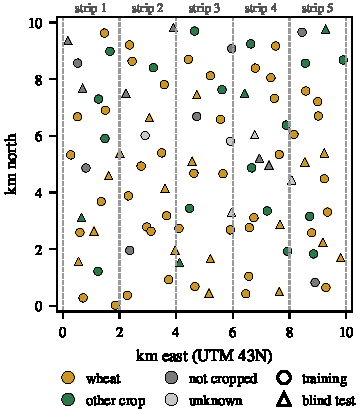
\includegraphics[width=0.78\columnwidth]{figures/study_area.pdf}
  \caption{\todo{caption: what is plotted, what to notice}}
  \label{fig:area}
\end{figure}

% ---------------------------------------------------------------------------------------------
\section{Labels and methods}
% about 0.75 page
% [ ] Sampling: one random point per km2 (seed 2026); outlines grown semi-automatically (one sentence).
% [ ] Three kinds of labels, the heart of the paper:
%     curve labels (k-means on NDVI curves, \NCurveLabels{} training fields);
%     blind labels from true colour only (\NClaudeLabels{} by an AI model at the author's request, \NNotFullyBlind{} not fully blind;
%       \NTestFromReview{} from the outline review);
%     farmer-confirmed labels from the field visit (\GroundN{} fields; how you asked, how sure).
% [ ] Classes merged into wheat / other crop / not cropped; \NTrain{} training and \NTest{} test fields.
% [ ] Features: \NFeatB{} hand-made (list in one sentence) vs raw 5-day curves.
% [ ] Models: logistic regression \cite{pedregosa2011sklearn}; MLP; TempCNN \cite{pelletier2019tempcnn};
%     U-Net \cite{ronneberger2015unet} with sparse and pseudo-labels; Presto \cite{tseng2023presto} frozen + linear probe.
% [ ] Evaluation: leave-one-strip-out spatial CV, settings tuned inside the training strips; one-SE rule \cite{hastie2009esl};
%     blind test opened once; balanced accuracy.
\todo{methods}

% ---------------------------------------------------------------------------------------------
\section{Results}
% about 1.25 pages, Table~\ref{tab:eval}, Table~\ref{tab:size}, Fig.~\ref{fig:confusion}, Fig.~\ref{fig:few}
% [ ] The same model, three evaluations: \CVAcc{} (\CVCorrect/\NTrain) on curve labels, \TestAcc{} (\TestCorrect/\NTest,
%     $\pm$\TestMargin) on blind labels, \GroundTestModel{} against farmers; baseline \BaselineTest.
% [ ] How the labels themselves held up against the farmers: blind \GroundTestLabels, curve \GroundTrainLabels.
% [ ] Model size (Table~\ref{tab:size}): MLP \MlpBal, TempCNN \TempcnnBal, U-Net \UnetSparseBal{} (sparse) and
%     \UnetPseudoBal{} (pseudo-labels), Presto \PrestoBal{} vs \CVBal{} for 51 weights.
% [ ] Few labels (Fig.~\ref{fig:few}): with 3 fields per fold, Presto \FewThreePresto{} vs \FewThreeRaw{} without pretraining
%     vs \FewThreeHand{} hand-made; with \FewTopSize: \FewTopPresto, \FewTopRaw, \FewTopHand.
\todo{results}

\begin{table}[t]
  \centering
  \caption{\todo{caption: one model, three evaluations}}
  \label{tab:eval}
  \footnotesize\setlength{\tabcolsep}{4pt}
  \begin{tabular}{lrr}
\toprule
Evaluated against & $n$ & Accuracy \\
\midrule
Curve-derived labels (spatial CV) & 68 & 99\% \\
Blind labels from true colour & 27 & 89\% \\
Farmer-confirmed (test fields) & \pending{n} & \pending{acc.} \\
\bottomrule
\end{tabular}

\end{table}

\begin{table}[t]
  \centering
  \caption{\todo{caption: spatial CV balanced accuracy on the training fields, by model size}}
  \label{tab:size}
  \footnotesize\setlength{\tabcolsep}{4pt}
  \begin{tabular}{lrr}
\toprule
Model & Weights & Bal.\ acc. \\
\midrule
Logistic regression, 16 features & 51 & 98\% \\
MLP, 16 features & 5{,}443 & 97\% \\
TempCNN, raw 5-day curves & 212{,}547 & 96\% \\
U-Net, sparse labels & 119{,}587 & 90\% \\
U-Net, + pseudo-labels & 119{,}587 & 98\% \\
Presto (frozen) + logistic & 404{,}160 & 93\% \\
\bottomrule
\end{tabular}

\end{table}

\begin{figure}[t]
  \centering
  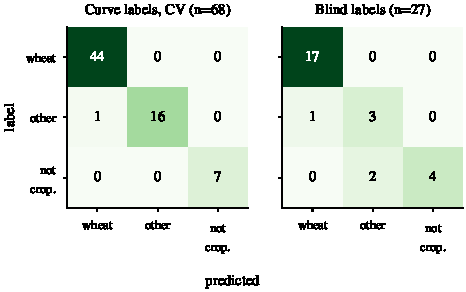
\includegraphics[width=\columnwidth]{figures/confusion.pdf}
  \caption{\todo{caption}}
  \label{fig:confusion}
\end{figure}

\begin{figure}[t]
  \centering
  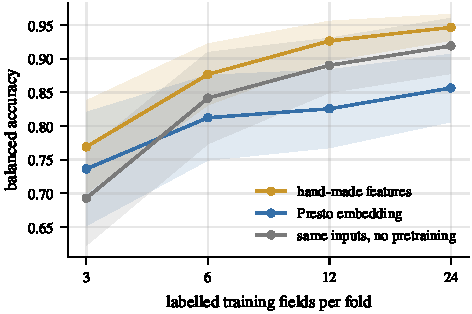
\includegraphics[width=\columnwidth]{figures/few_labels.pdf}
  \caption{\todo{caption: mean and spread over 30 random draws per size}}
  \label{fig:few}
\end{figure}

% ---------------------------------------------------------------------------------------------
\section{Discussion and limitations}
% about 0.5 page
% [ ] Why CV flattered: the labels came from the curves the model learns from.
% [ ] What the farmers' answers add (and where they disagreed with the blind labels).
% [ ] Why bigger models did not help: few labels; the crop calendar is simple and the hand-made features encode it.
% [ ] Limitations, briefly: one area and one season; \NTest{} test fields ($\pm$\TestMargin{} points);
%     Presto missing red edge, SWIR, weather and elevation; probed, not fine-tuned.
\todo{discussion}

% ---------------------------------------------------------------------------------------------
\section{Conclusion}
% about 0.2 page: the claim with its three key numbers, and the next step (second season; flood crop damage).
\todo{conclusion}

% ---------------------------------------------------------------------------------------------
\section*{Acknowledgment}
% Write in your own words:
% [ ] Copernicus Sentinel data, Planetary Computer.
% [ ] People who helped (the farmers; advisors who are not co-authors).
% [ ] AI use, plainly: code written with an AI coding assistant; \NClaudeLabels{} blind labels made by an AI model;
%     the text written by the author. (IEEE requires disclosure of AI-generated content.)
\todo{acknowledgment}

\nocite{*} % lists every reference while the text has no \cite yet: delete once you cite them
\bibliographystyle{IEEEtran}
\bibliography{references}

\end{document}
